\chapter{Обзор предметной области}
\label{chapter1}

\section{Основные понятия}

Биоинформатика \cite{scala_lang} — это наука на стыке двух дисциплин: биологии и информатики. Многие задачи биологии требуют обработки колоссального объема данных, что и привело к возникновению дисциплины. Одной из важных задач биоинформатики является задача корректной оценки собранной геномной последовательности.

\subsection{Строение ДНК}

\textit{Геном} — это совокупность информации, передаваемой всеми живыми существами по наследству. Геномы большинства живых организмов состоят из молекул \textit{ДНК} — дезоксирибонуклеиновой кислоты. ДНК — это полимерная молекула, представляющая из себя две закрученных цепочки, состоящие из соединённых в последовательность \textit{нуклеотидов}. Нуклеотиды, входящие в ДНК, разделяют по азотистым основаниям на четыре группы: \textit{аденин} (A), \textit{цитозин} (C), \textit{гуанин}(G),  и \textit{тимин} (T). Цепи ДНК соединены между собой по \textit{принципу комплиментарности}: аденин с тимином, цитозин с гуанином.

Геном в биоинформатике представляется одной из двух комплементарных  цепей молекулы ДНК. Строка, состоящая из символов A, G, C и T, соответвующих типам нуклеотидов,является наиболее удобным представлением генома в биоинформатике.


\subsection{Секвенирование генома}

Для определения линейной последовательности нуклеотидов в молекуле ДНК геном подвергают секвенированию. Одним из популярных методов секве-нирования является метод дробовика (Shotgun Sequencing). Метод состоит в выделении из молекулы ДНК коротких участков (порядка нескольких сотен последовательных нуклеотидов), после чего происходит посимвольное считывание концов выделенных участков. Таким образом, получаются парные чтения (mate-pairs). В силу множества различных факторов при прочтении от-дельных нуклеотидов могут быть допущены ошибки. Также неизвестно точное расстояние между чтениями, известно лишь распределение длин фрагментов.

\subsection{Сборка генома}

Традиционно процесс сборки генома состоит из трех этапов: исправление ошибок в парных чтениях, сборка контигов, длинных последовательных частей геномной последовательности, и сборка скэффолдов, наборов упорядо-ченных ориентированных контигов с оценками расстояния между соседними контигами. Таким образом, задачей сборки скэффолдов является построение вышеупомянутых наборов по множеству контигов и библиотекам парных чтений. Про библиотеки парных чтений известны математическое ожидание и стандартное отклонение длин фрагментов, из которых были получены парные чтения.


\section{Постановка задачи}

В последнее время появилось множество сборщиков генома. Возникла проблема сравнения качества их работы. В прошлом это делалось при помощи таких популярных метрик как \textit{N50/N90}, \textit{NG50/NG90}, длина наибольшего контига или скэффолда.  Хотя исследования показали, что простые метрики коррелируют с качеством сборки, используемые в настоящее время метрики являются грубыми и не обеспечивают полной информации о результате сборки.
\begin{figure}[t]
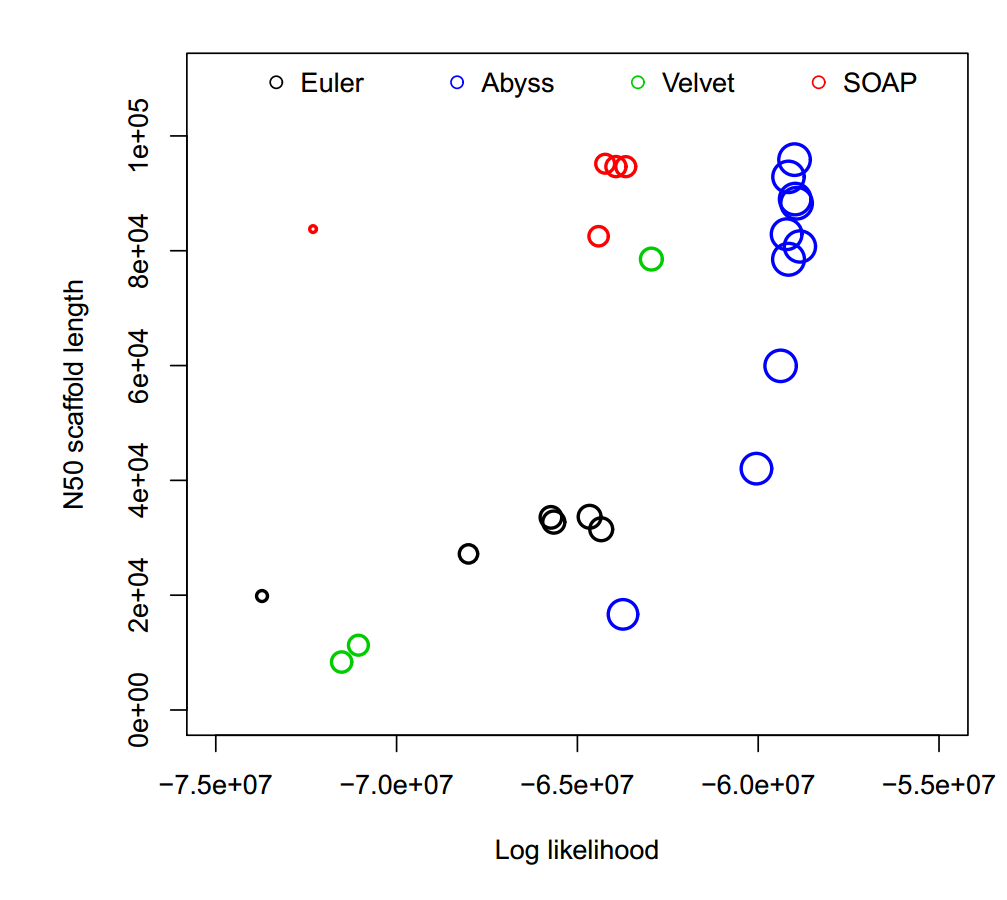
\includegraphics[scale=0.25]{fig1.png}
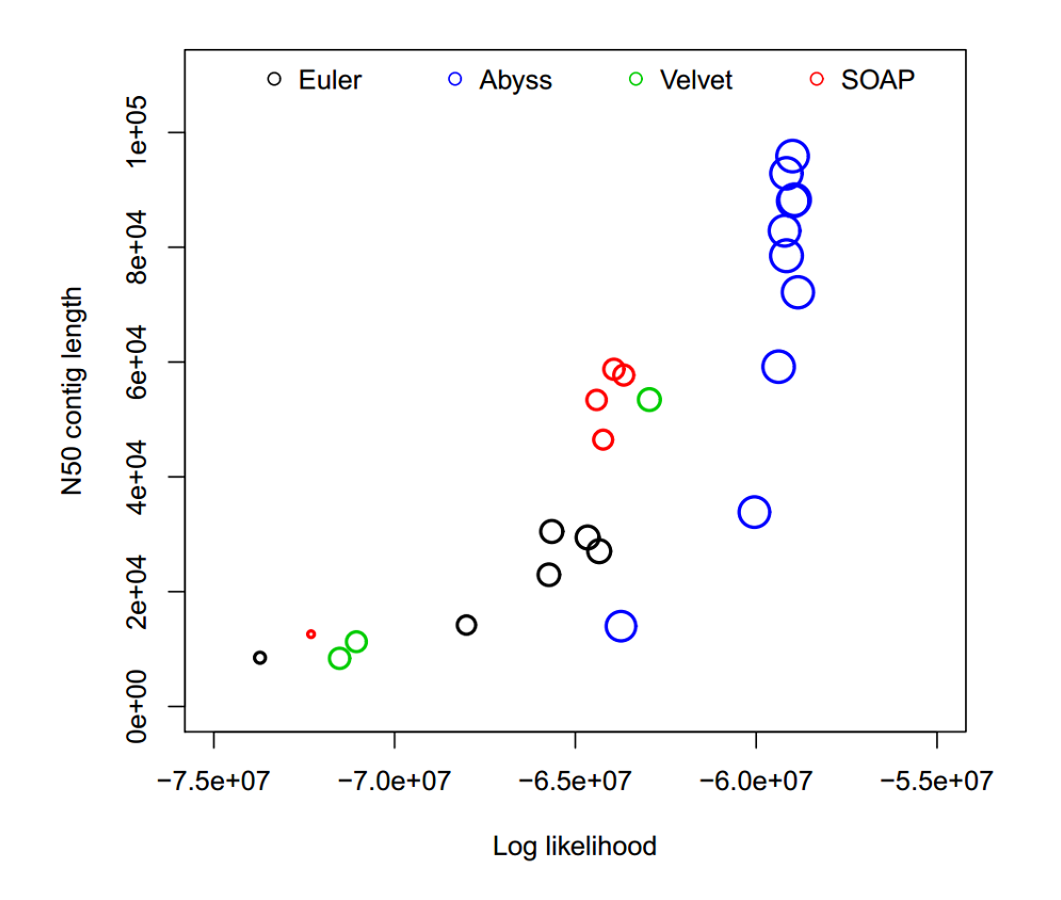
\includegraphics[scale=0.25]{fig2.png}
\caption{Графики корреляции N50 и loglikelihood, посчитанным с помощью CGAL, для \textit{E.coli}. Окружности соответствуют сборкам с различными длинами k-меров. Размер окружности соответствует схожести с эталонной сборкой.}
\label{fig:N50vsLoglik}
\end{figure}
Например сборка, состоящая из просто склеенных конец-в-конец чтений, имеет очень большой \textit{N50}, но, очевидно, плохое качество сборки.

Требуется разработать метрику, качественно оценивающую сборку на основе принципа максимального правдоподобия.


\section{Обзор существующих методов и их проблем}
За последние два года было разработано несколько новых способов качественной оценки сборки геномной последовательности на основе принципа максимального правдоподобия. Их способ заключается в получении \textit{loglikelihood} -- логарифма вероятности того, что сборка является верной при наличии заданного набора чтений.

\subsection{CGAL}
Данный метод является первым методом оценки на основе принципа максимального правдоподобия. В её основе лежит слудующая формула:

$$l(A,R)=\ln \prod_{i=1}^n p(r_i|A)\approx \sum_{i=1}^N \ln\sum{j=1}^M_i p_F(l_{i,j})p_S(s_{i,j})p_E(r_i|a_{i,j}, e_{i,j})$$

\begin{itemize}
\item $R$ -- множество чтений;
\item $A$ -- сборка;
\item $M_i$ -- количество возможных "соответствий" в сборке чтения $r_i$;
\item $l_{i,j}$, $s_{i,j}$, $a_{i,j}$ и $e_{i,j}$ -- соответственно длина чтения, позиция чтения, подпоследовательность сборки и ошибки для "соответствия" $j$ для чтения $i$.
\end{itemize}

Проблема данного метода заключается в том, что согласно авторам данного метода чтения должны быть распределены равномерно по всей длине генома, что является существенным недостатком, поскольку в реальной ситуации чтения распределены чаще всего неравномерно.

\subsection{de Novo}
В основе данного метода лежит формула Байеса:

$$P(A|R)=\frac{P(R|A)P(A)}{P(R)}$$

$A$ -- событие, при котором сборка является эталонной геномной последовательностью $R$ -- событие, при котором исследуется определённый набор чтений. $P(A)$ и $P(R)$ являются константами.

$$P(R|A)=\prod_{r\in R}P(r|A)$$


Задача сводится к получению оценки $P(r|A)$ с использованием  динамического программирования. Данный метод достаточно точно вычисляет вероятности ошибок для больших наборов чтений. Однако существенными недостатками являются большой объём потребляемой памяти ($O(n^2)$, где $n$ -- длина сборки) и сложность в реализации данного алгоритма. Кроме того на сегодняшний день нет ни одной работающей реализации данного подхода.


\subsection{ALE}
На данный момент этот метод является наиболее совершенным. В его основе также лежит формула Байеса, как и в \textit{de Novo}.
$$P(A|R)=\frac{P(R|A)P(A)}{Z}$$
$Z$ – константа.
$P(A)$ описывает качество сборки в отсутствие какой-либо информации о чтениях.
$P(R|A)$ оценивается по следующей формуле:
$$P(R|A)=P_{placement}(R|A)P_{insert}(R|A)P_{depth}(R|A)$$

$P_{placement}$ оценивает, насколько хорошо содержание чтений совпадает со сборкой, $P_{insert}(r|A)$ оценивает, насколько хорошо 
априорные расстояния между парными чтениями (insert length) совпадают с получившимися в результате сборки, $P_{depth}(r|A)$ оценивает, насколько априорная глубина покрытия в каждой позиции совпадает с получившейся в результате сборки на основе GC-контента. \textit{Глубина покрытия} – это количество чтений, которое покрыло данную позицию в сборке. \textit{GC-контент} – это процентный состав суммы всех нуклеотидов, являющихся гуанином(G) или цитозином(C) по отношению к длине исследуемого участка генома.

Более подробно о данном методе и о его проблемах будет изложено в следующей главе.

\section{Выводы к главе 1}
В условиях быстро появляющихся новых сборщиков, возникла задача качественного сравнения их между собой, поэтому разработка метрики оценки качества сборки геномной последовательности является важной задачей биоинформатики. Существующие популярные метрики, такие как \textit{N50/N90}, не дают полной информации о результате сборки, поэтому был предложен новый подход, заключающийся в вычислении \textit{loglikelihood} -- логарифма вероятности того, что сборка является верной при заданном наборе чтений.
В последнее время было предложено несколько способов получения \textit{loglikelihood}, однако они не лишены своих недостатков. Наиболее совершенным инструментом оценки на сегодняшний день является ALE. В данной работе представлен способ оценки качества на базе ALE.